\documentclass{implementierungsheft}
% glossary
\makeglossaries

\begin{document}
\newglossaryentry{label}{
    name=Label,
    plural=Labels,
    description={Rezepte können mit bezeichnenden Stichwörtern, sogenannten Labels, versehen werden. Dies ermöglicht das Filtern von Rezepten nach bestimmten Eigenschaften (z.B. vegetarisch, glutenfrei, halal)}
}
\maketitle
\tableofcontents
\newpage

\section*{Gender-Hinweis}
Zur besseren Lesbarkeit wird in diesem Entwurfsheft das generische Maskulinum verwendet.
Die in diesem Heft verwendeten Personenbezeichnungen beziehen sich - sofern nicht anders kenntlich gemacht - auf alle Geschlechter.
\newpage

\section{Umsetzung der Zielbestimmungen des Pflichtenhefts}
Es wurden alle Muss-, Soll- und Kannkriterien umgesetzt. Die Applikation wurde um die Folgenden Features erweitert:
\begin{itemize}
    \item An sinnvollen Stellen wurden zusätzliche Pop-Up-Fenster eingefügt, die z.B. nach Bestätigung einer Aktion fragen.
    \item Es gibt eine weitere Ansicht, die die exportierten Rezepte als PDF-Vorschau anzeigt.
    \item Die App ist je nach Systemsprache auf Deutsch oder Englisch übersetzt.
\end{itemize}
\newpage
\section{Änderungen am Entwurf}
In den folgenden UML-Diagrammen werden abgeänderte Methoden und Attribute blau markiert, entfernte rot und neue grün.
\subsection{Änderungen am Modellayer}
\begin{figure}[htp]
    \centering
    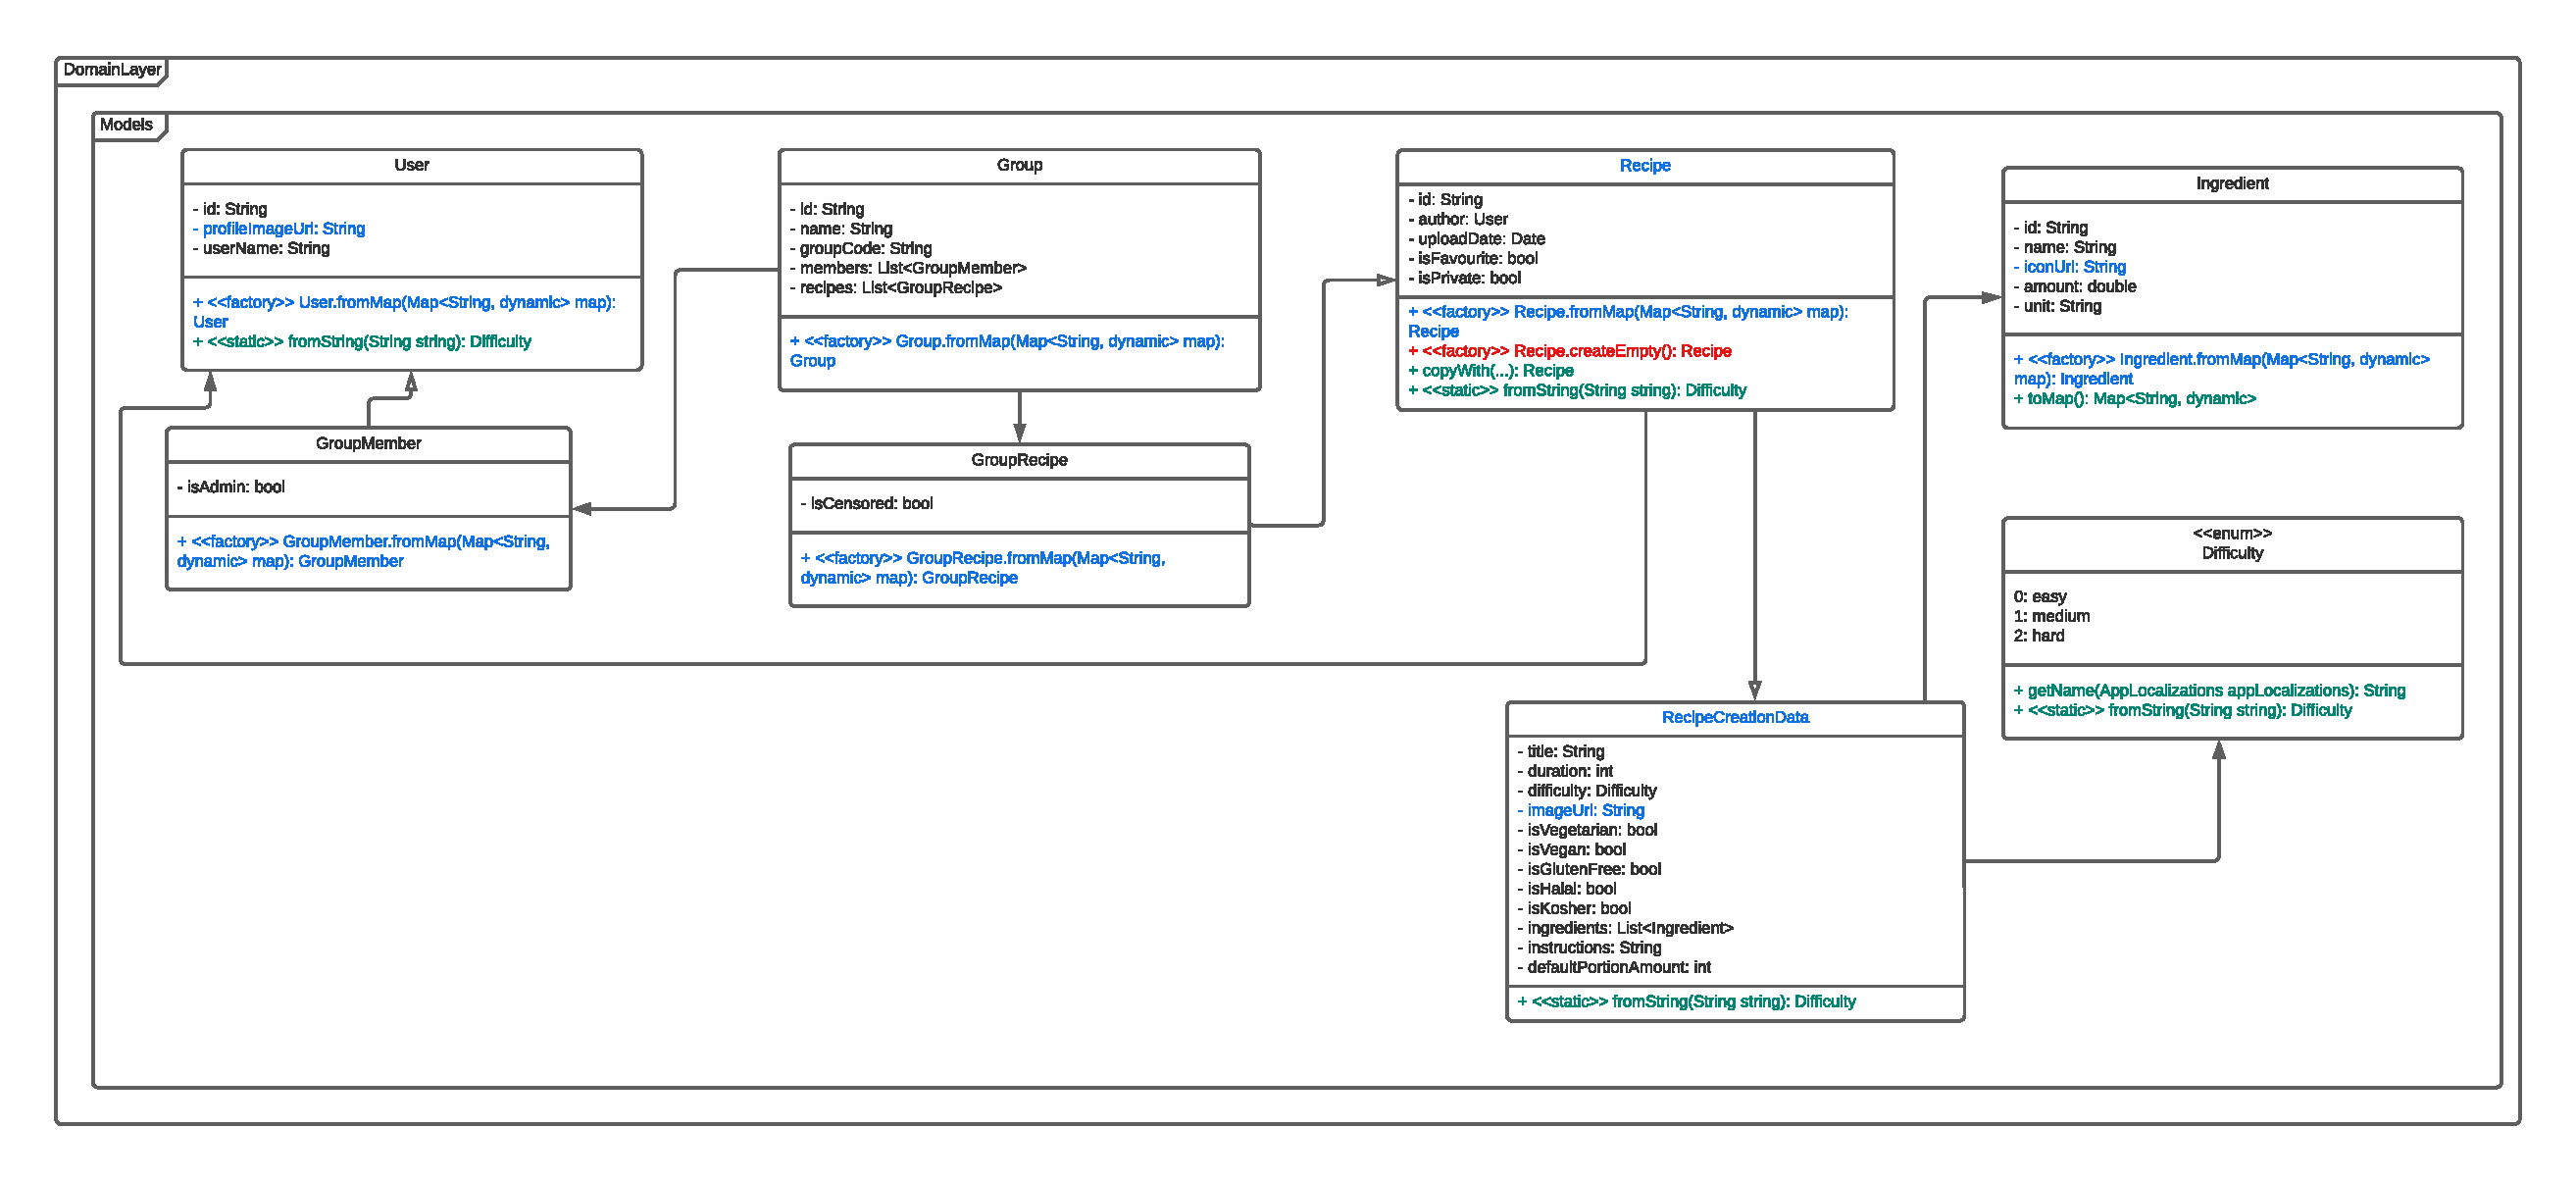
\includegraphics[width=\textwidth]{images/uml/modelLayer.pdf}
    \caption{Änderungen am Modellayer}
    \label{fig:modellayer}
\end{figure}
\paragraph*{\texttt{fromMap(Map<String, dynamic> map)}} Die Factory-Methoden \texttt{fromJson} wurden in \texttt{fromMap} umbenannt, da sie unabhängig von der Serialisierungsmethode sind.
\paragraph*{\texttt{toMap()}} Die statische Methode \texttt{toMap} wurde bei einigen Klassen hinzugefügt, um die Serialisierung zu vereinfachen. Sie gibt ein \texttt{Map<String, dynamic>} zurück, das die Attribute der Klasse enthält.
\paragraph{\texttt{Recipe} und \texttt{RecipeCreationData}}
Die Klasse \texttt{Recipe} wurde in die beiden Klassen \texttt{Recipe} und \texttt{RecipeCreationData} aufgeteilt. Die Klasse \texttt{Recipe} enthält nur noch die Attribute, die ein Rezept nach der Erstellung haben kann, wie zum Beispiel den Author und die Id. Die Klasse erbt von \texttt{RecipeCreationData}, die die Attribute enthält, die ein Rezept bei der Erstellung haben muss, wie Namen oder Anweisungen.
\paragraph{\texttt{Recipe.copyWith(...)}} Die Methode \texttt{copyWith} wurde hinzugefügt, um ein Rezept zu kopieren und dabei einzelne Attribute zu ändern. Die zuändernden Attribute werden als benannte Parameter übergeben.
\paragraph{\texttt{Recipe.createEmpty()}} Die Methode wurde entfernt, da sie nicht mehr benötigt wird.
\paragraph{\texttt{Difficulty.getName(AppLocalizations appLocalizations): String}}
Die Methode gibt einen String zurück, der den Namen der Schwierigkeit in der aktuellen Sprache enthält. Die Sprache wird aus den \texttt{AppLocalizations} gelesen.
\paragraph{\texttt{Difficulty.fromString(String string)}}
Die statische Methode gibt die Schwierigkeit zurück, die den übergebenen String als Namen hat.
\paragraph{\texttt{RecipeCreationData.imageUrl} und \texttt{Ingredient.iconUrl}} Wir haben uns dazu entschieden statt dem Icon/Bild selbst nur die URL zu speichern. Damit können wir die Anfragengröße massiv verkleinern. Mehr dazu folgt im Kapitel \ref{sec:images}.
\newpage
\subsection{Änderungen am Datalayer}
\begin{figure}[htp]
    \centering
    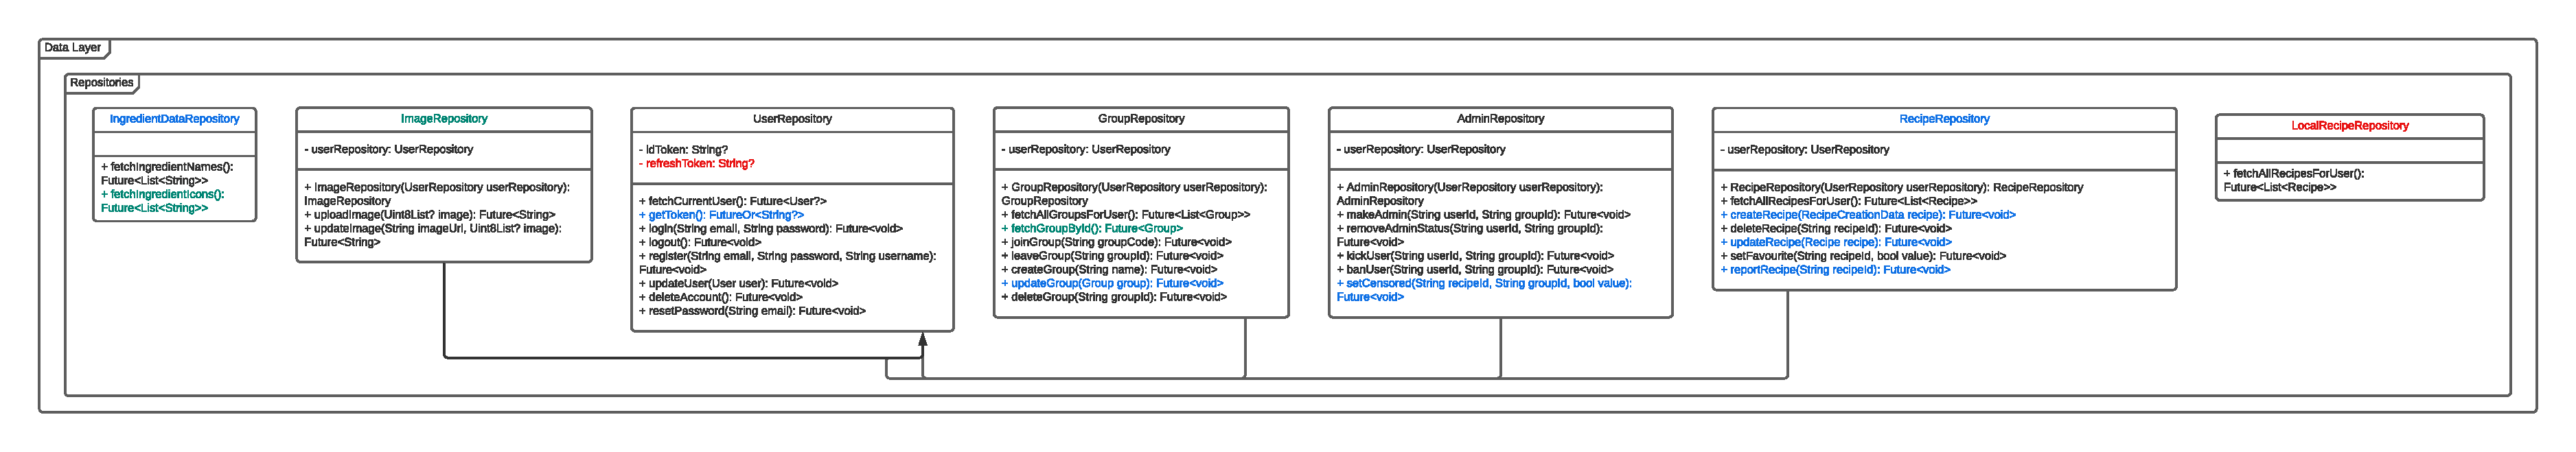
\includegraphics[width=\textwidth]{images/uml/dataLayer.pdf}
    \caption{Änderungen am Datalayer}
    \label{fig:dataLayer}
\end{figure}
\subsubsection{\texttt{RecipeRepository}}
Das Konzept, ein lokales und ein entferntes Repository zu haben, wurde verworfen. Stattdessen gibt es nur noch ein Repository, das auf die Daten des Servers zugreift.
\paragraph{\texttt{createRecipe(RecipeCreationData recipe)}} Die Methode nimmt statt einem \texttt{Recipe} ein Objekt der neuen Klasse \texttt{RecipeCreationData} entgegen, das wirklich nur die benötigten Daten enthält.
\paragraph{\texttt{updateRecipe(Recipe recipe)}} Die Methode nimmt keine Id mehr als Parameter entgegen. Stattdessen wird die Id aus dem übergebenen \texttt{Recipe} gelesen.
\paragraph{\texttt{reportRecipe(String recipeId)}} Die Methode nimmt nur noch die Id des zu meldenden Rezepts entgegen und nicht mehr das gesamte Rezept.
\subsubsection{\texttt{AdminRepository}}
\paragraph{\texttt{setCensored(String recipeId, String groupId, bool value)}} Im Entwurf wurde vergessen, die Id der Gruppe als Parameter hinzuzufügen. Das wurde nun nachgeholt.
\subsubsection{\texttt{GroupRepository}}
\paragraph*{\texttt{fetchGroupById()}} Die Methode wurde hinzugefügt, um eine Gruppe anhand ihrer Id zu laden. Dies ist vor allem für die Gurppen-Detail-Seite nötig.
\paragraph*{\texttt{updateGroup(Group group)}} Die Methode nimmt keine Id mehr als Parameter entgegen. Stattdessen wird die Id aus der übergebenen \texttt{Group} gelesen.
\subsubsection{\texttt{UserRepository}}
\paragraph{\texttt{refreshToken}}
Das Attribut wurde entfernt. Stattdessen wird das Token im Systemspeicher abgelegt, da es nur selten benötigt wird, aber über mehrere Sitzungen hinweg gültig ist.
\paragraph{\texttt{getToken(): FutureOr<String?>}} Die Methode gibt ein \texttt{FutureOr<String?>} zurück, da das Token asynchron geladen werden kann, jedoch nicht muss.
\subsubsection{\texttt{IngredientDataRepository}}
Die Klasse wurde umbenannt, da sie nun nicht mehr nur die Namensvorschläge für Zutaten enthält, sondern auch die für Icon-Urls.
\paragraph{\texttt{fetchIngredientIconUrls()}} Die Methode wurde hinzugefügt, um die Liste der möglichen Icons zu laden.
\newpage
\subsection{Änderungen am Domainlayer}
\begin{figure}[htp]
    \centering
    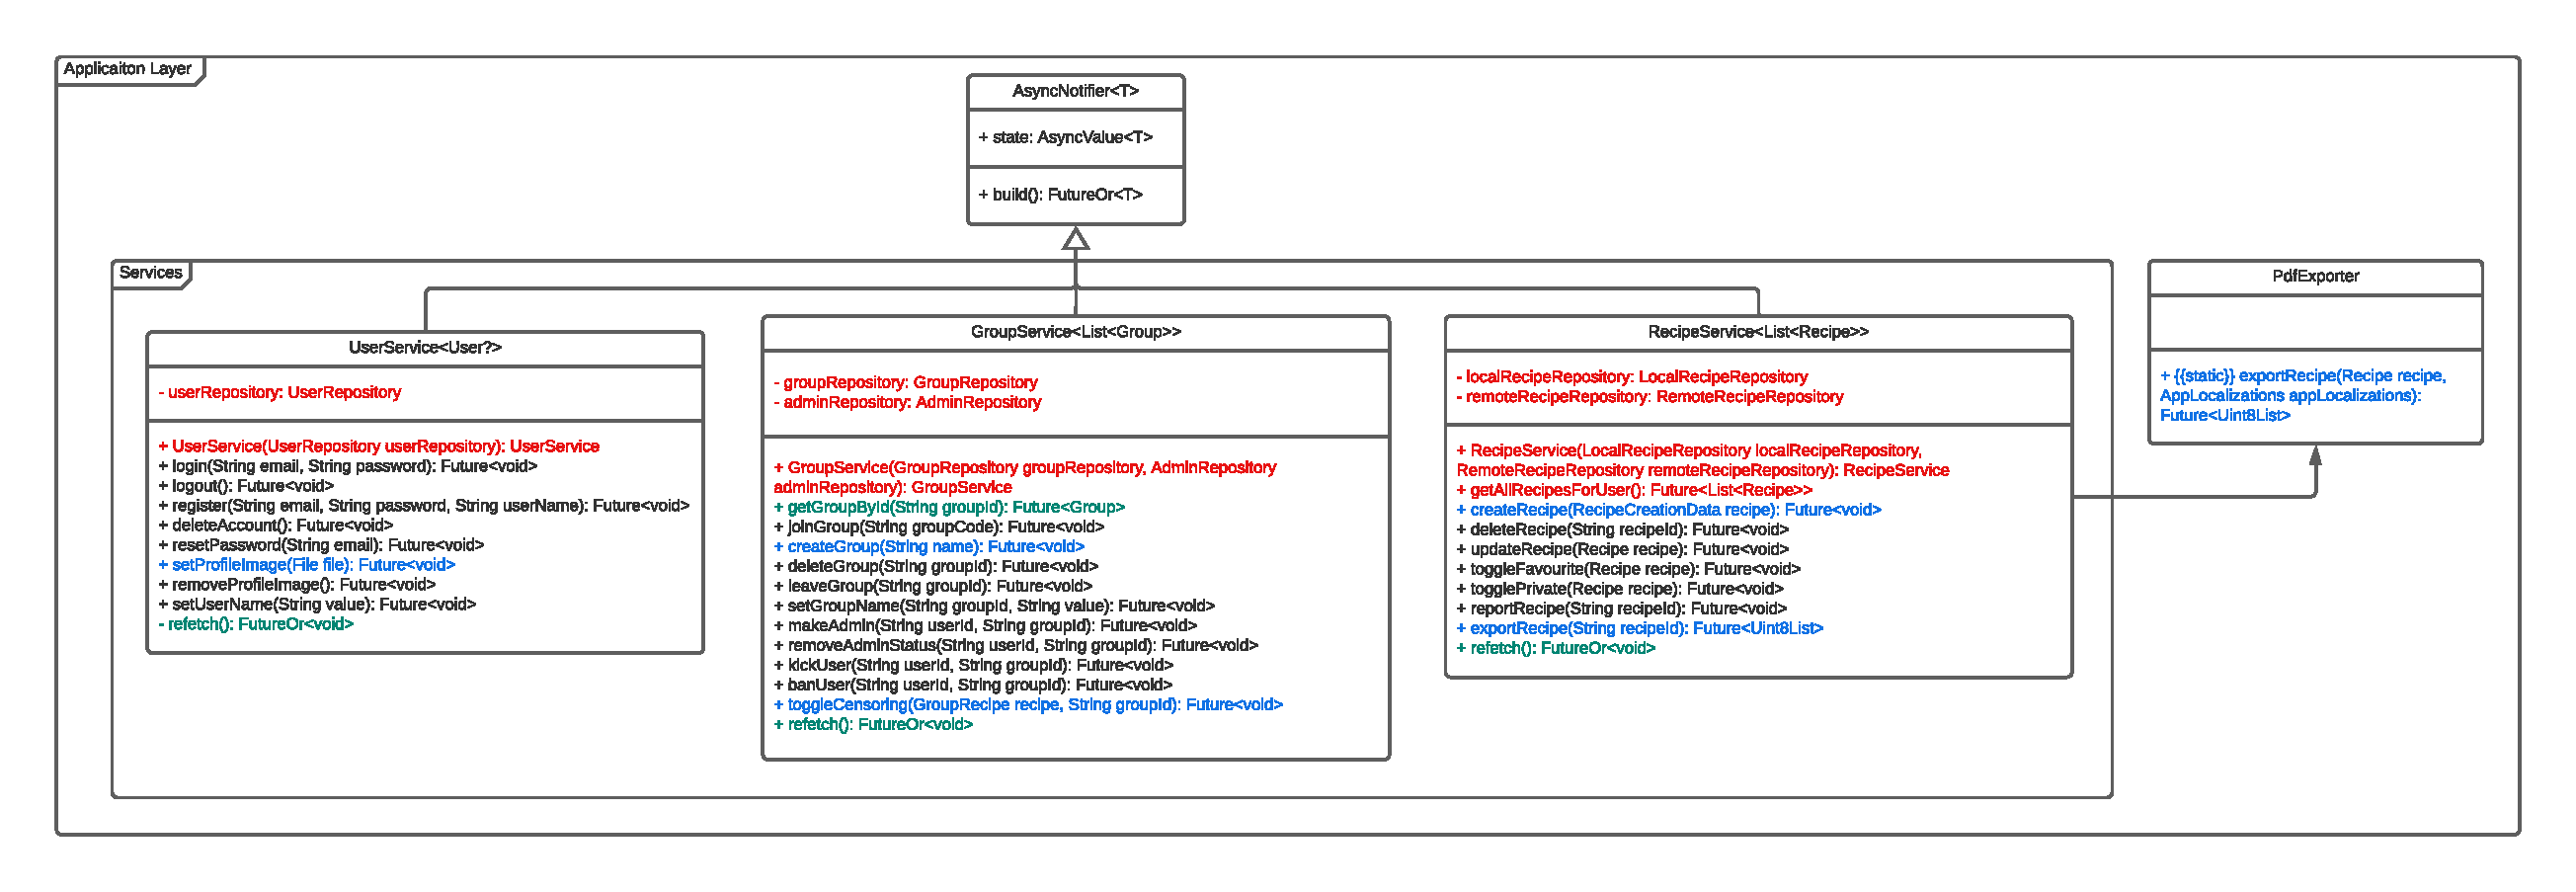
\includegraphics[width=\textwidth]{images/uml/domainLayer.pdf}
    \caption{Änderungen am Domainlayer}
    \label{fig:domainLayer}
\end{figure}
\paragraph{Repository-Objekte und Konstruktoren}
Da alle von \texttt{AsyncNotifier} erbenden Klassen Zugriff auf ein \texttt{ref} Objekt haben, benötigen sie keine Referenz auf die einzelnen Repositories mehr. Stattdessen können sie über dieses Objekt auf die Repositories zugreifen. Somit sind auch die Konstruktoren nicht mehr nötig und wurden entfernt.
\paragraph{\texttt{refetch()}}
Alle Services besitzen eine Methode \texttt{refetch()}, die die gehaltenen Daten neu lädt. Sie ist öffentlich, damit die Daten auch von außen neu geladen werden können. Die einzige Ausnahme bildet dabei der \texttt{UserService}, da dieser nur sich selbst neu laden können muss.
\subsubsection{\texttt{UserService}}
\paragraph*{\texttt{setProfileImage(File file)}}
Der Name des Parameters wurde von \texttt{image} zu \texttt{file} geändert, um zu verdeutlichen, dass es sich um eine Datei handelt. Ansonsten wurde die Methode nicht geändert.
\subsubsection{\texttt{GroupService}}
\paragraph*{\texttt{getGroupById(String groupId)}}
Die Methode wurde hinzugefügt, um eine Gruppe anhand ihrer Id zu laden. Dies ist vor allem für die Gurppen-Detail-Seite nötig.
\paragraph{\texttt{createGroup(String name)}}
Der Parameter wurde von \texttt{title} zu \texttt{name} geändert, um Konsistenz zum Repository zu haben.
\paragraph{\texttt{toggleCensoring(GroupRecipe recipe, String groupId)}}
Der Typ des \texttt{recipe} Parameters wurde von \texttt{Recipe} zu \texttt{GroupRecipe} geändert. Dies ist nötig um Zugriff auf das \texttt{isCensored} Attribut zu haben und entsprechend die richtige Anfrage zu stellen.
\subsubsection{\texttt{RecipeService}}
\paragraph{\texttt{getAllRecipesForUser()}}
Die Methode war fälschlicherweise noch im Entwurf vorhanden. Sie wurde aber durch die \texttt{build()} Methode ersetzt.
\paragraph{\texttt{createRecipe(RecipeCreationData recipe)}}
Es wird die neue Klasse \texttt{RecipeCreationData} verwendet, die nur die benötigten Daten enthält.
\paragraph{\texttt{exportRecipe(String recipeId)}}
Die Klasse gibt nun ein \texttt{Future<Uint8List>} zurück, das die Daten des PDFs enthält. Dies ermöglicht es die Daten anschließend in einer Preview anzuzeigen.
\subsubsection{PDFExporter}
\paragraph{\texttt{exportRecipe(Recipe recipe, AppLocalizations appLocalizations)}}
Es wird nun auch ein \texttt{AppLocalizations} Objekt entgegengenommen, um die Übersetzungen zu laden. Zudem gibt sie auch ein \texttt{Future<Uint8List>} zurück, das die Daten des PDFs enthält. Dies ermöglicht es die Daten anschließend in einer Preview anzuzeigen.
\newpage
\subsection{Änderungen am Presentationlayer}
\begin{figure}[htp]
    \centering
    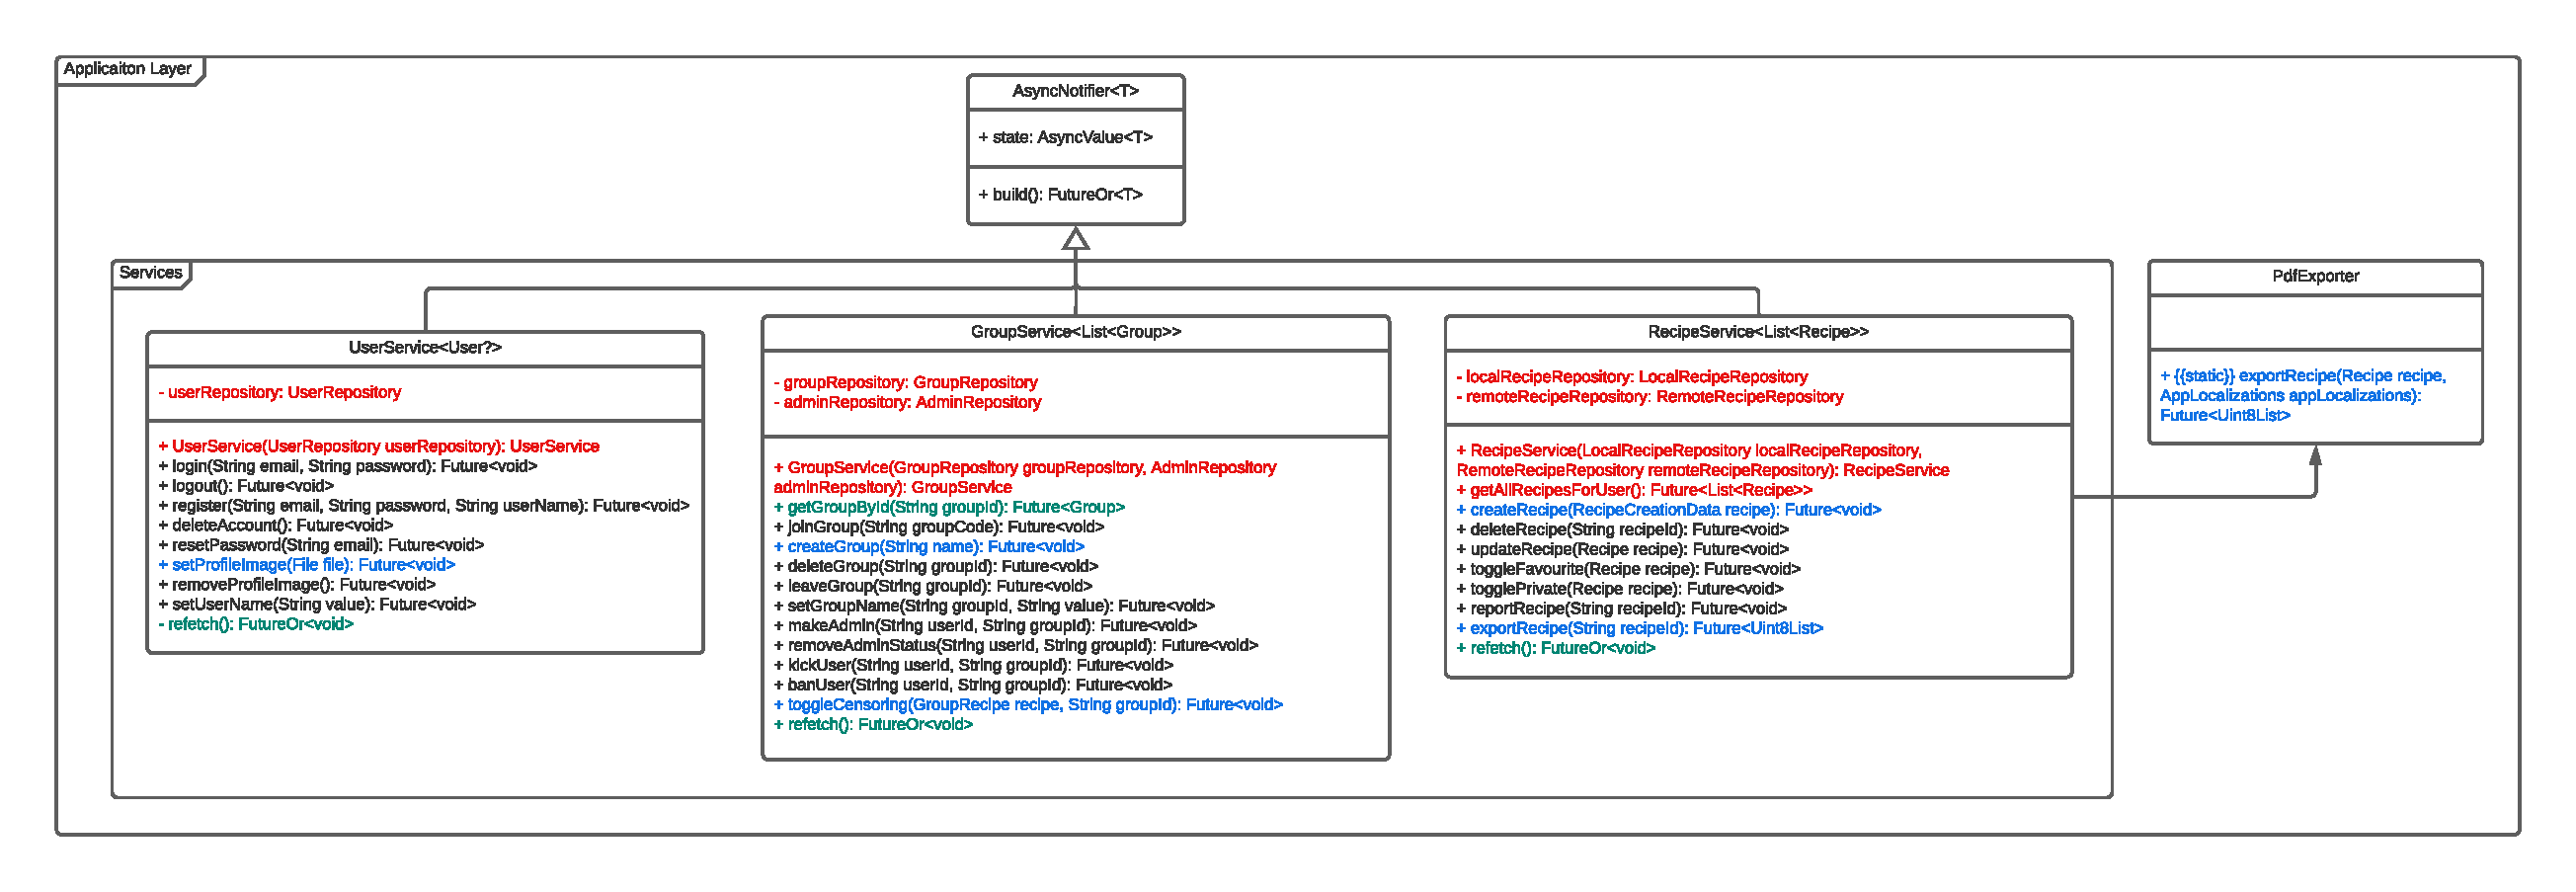
\includegraphics[width=\textwidth]{images/uml/domainLayer.pdf}
    \caption{Änderungen am Presentationlayer}
    \label{fig:presentationLayer}
\end{figure}
Alle Attribute der Klassen werden in einem Konstruktor gesetzt, der der Übersichtlichkeit halber nicht dargestellt wird. Die Ausnahme bilden die Attribute, die als Zustand der \texttt{StatefulWidgets} gehalten werden. Sie sind daran zu erkennen, das sie \textit{kursiv} geschrieben sind.
\paragraph{Vererbungen}
Google selbst empfiehlt für Flutter-Widgets keine Vererbung von anderen Widgets zu verwenden. Stattdessen soll die \texttt{build}-Methode des Widgets alle nötigen Anpassungen vornehmen. Dieses Prinzip nennt sich "Composition over Inheritence". Daher wurden die Vererbungen zu Klassen wie \texttt{IconButton} entfernt.
\paragraph{\texttt{ConsumerWidget} und \texttt{ConsumerStatefulWidget}} Die beiden Klassen aus dem \texttt{Riverpod}-Paket wurden an sinnvollen Stellen verwendet, um die Daten aus den Providern laden zu können.
\section{Glossar}
\printglossary[style=altlist]
\end{document}